\documentclass{article}

\usepackage{graphicx}
\usepackage{tikz}
\usepackage{tikzsymbols}
\usetikzlibrary{calc,patterns,shapes.geometric}
\pagestyle{empty}
\usepackage[margin=0pt]{geometry}
\geometry{papersize={14in,12in}}

\def\centerarc[#1](#2)(#3:#4:#5){\draw[#1] ($(#2)+({#5*cos(#3)},{#5*sin(#3)})$) arc (#3:#4:#5);}

\begin{document}
	\begin{figure}
		\centering
		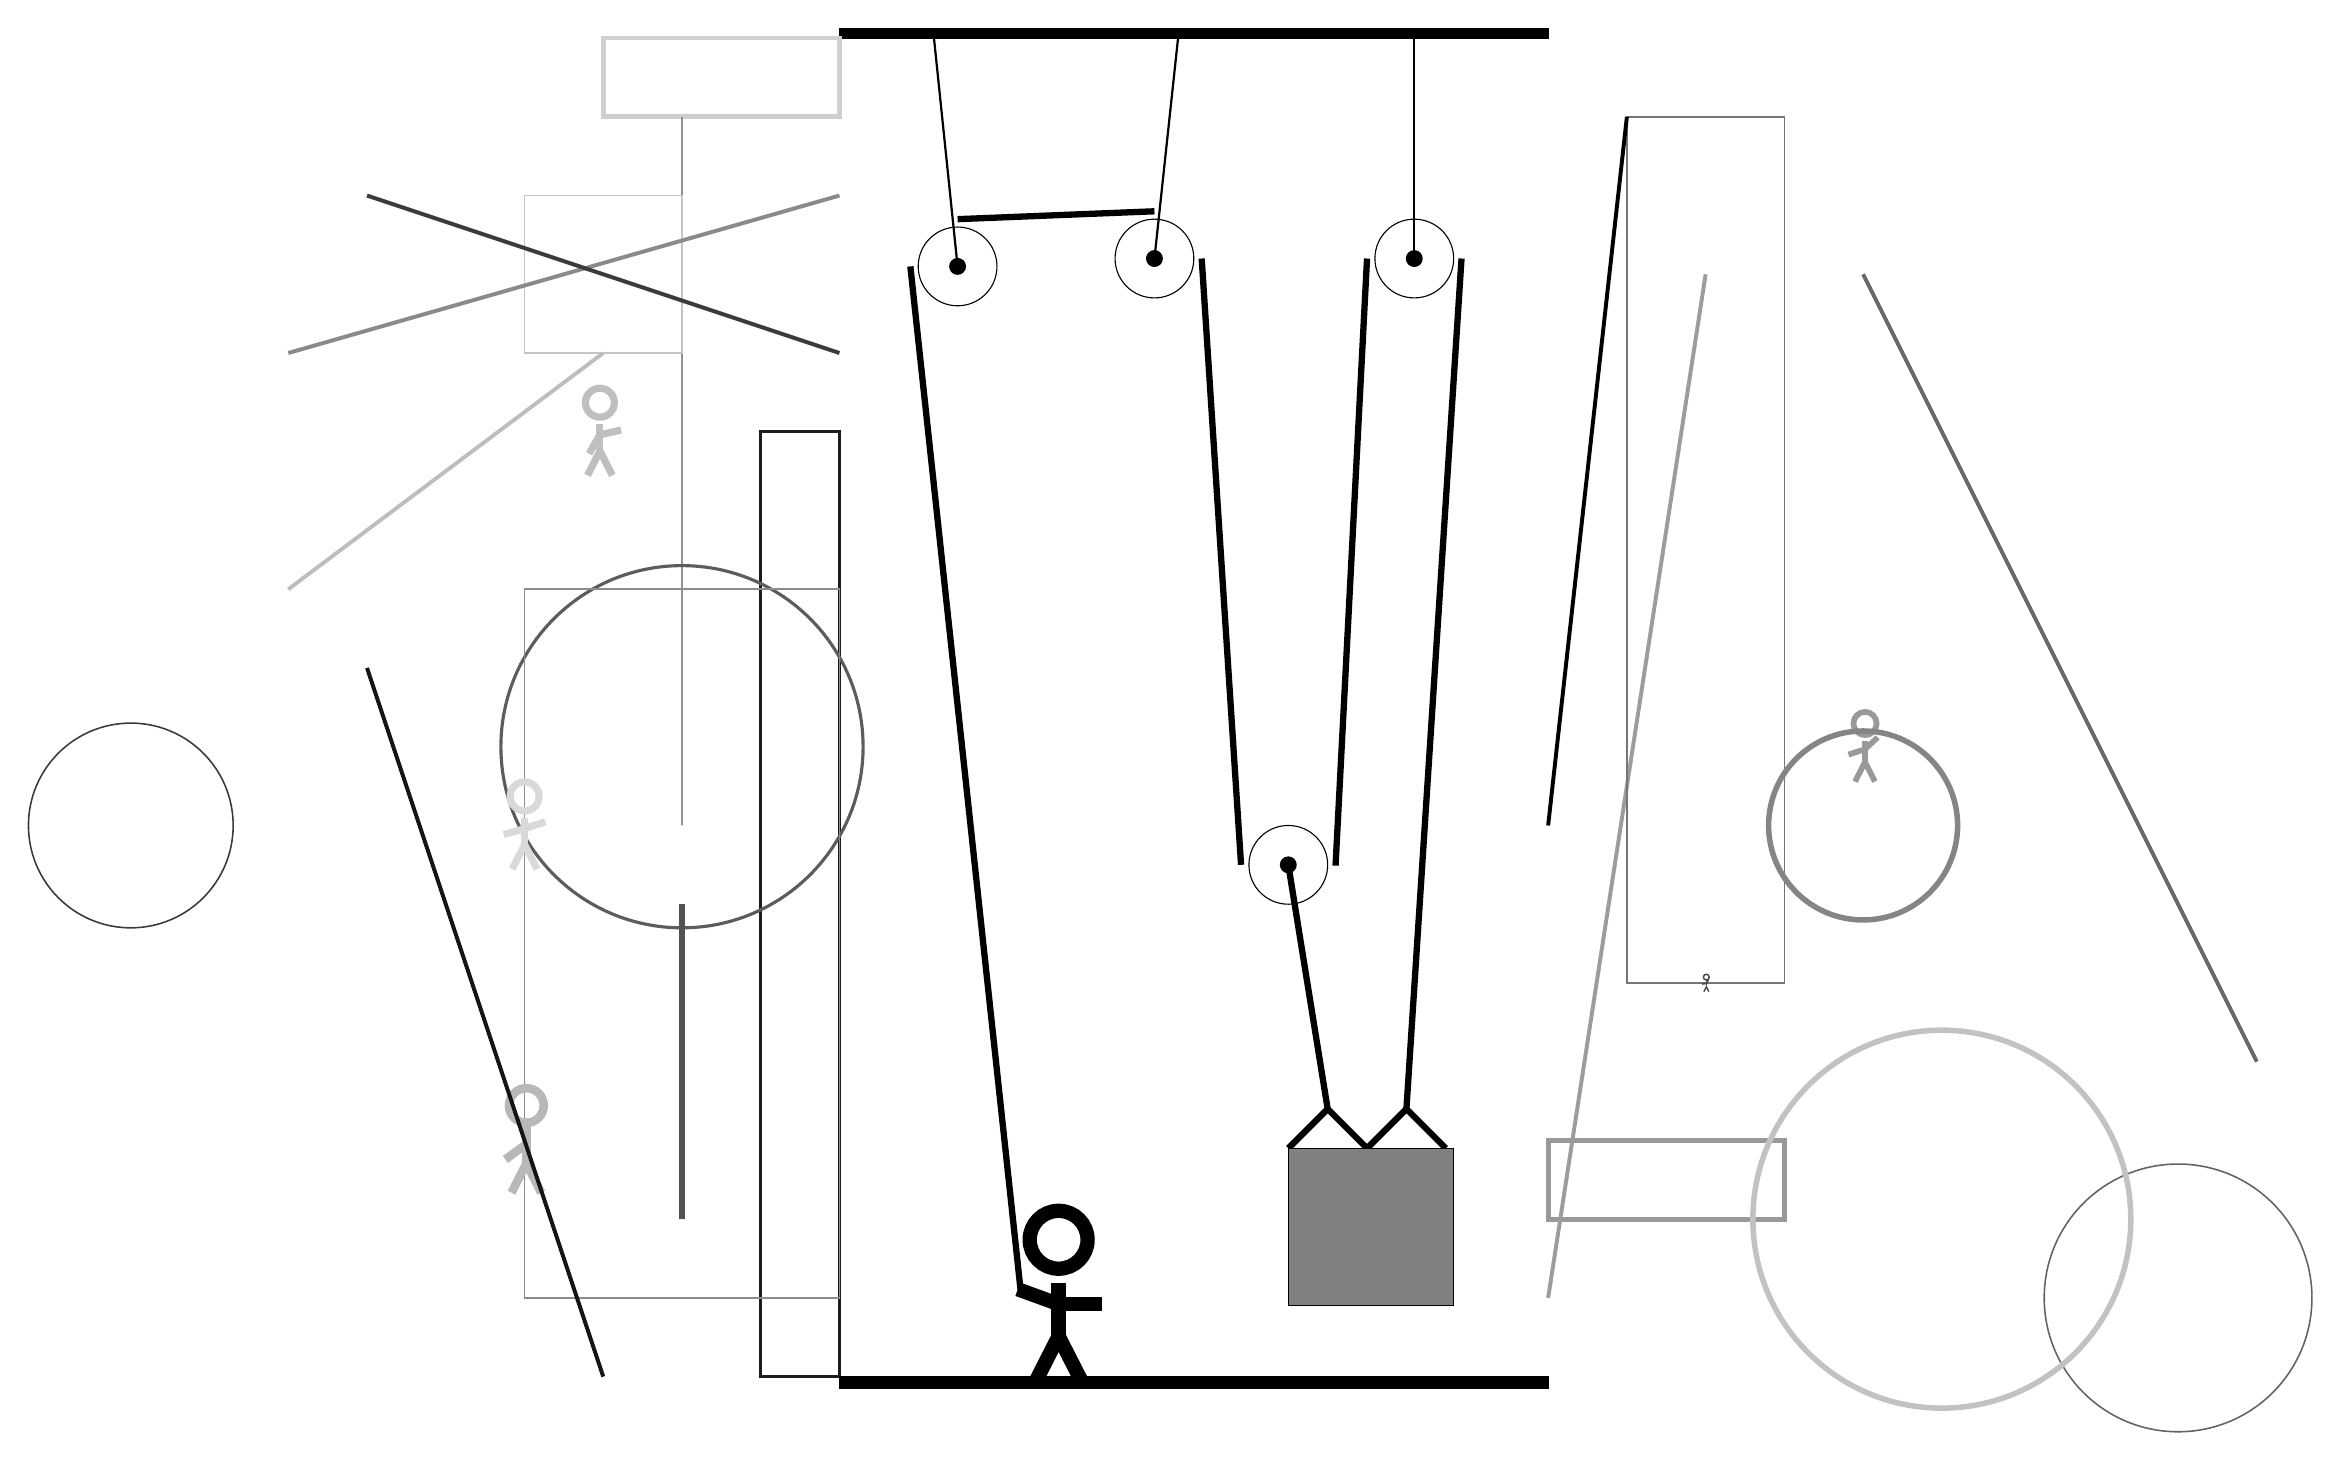
\begin{tikzpicture}
			%%%%% START %%%%%
			
			\draw[fill=black] (-3, 14) rectangle (6, 14.125);
			
			\draw (1, 11.2) circle (0.5);
			\draw[fill=black] (1, 11.2) circle (0.1);
			\draw[thick] (1, 11.2) -- (1.3, 14);
			
			\draw (4.3, 11.2) circle (0.5);
			\draw[fill=black] (4.3, 11.2) circle (0.1);
			\draw[thick] (4.3, 11.2) -- (4.3, 14);
			
			\draw (2.7, 3.5) circle (0.5);
			\draw[fill=black] (2.7, 3.5) circle (0.1);
			
			\draw[line width=0.8mm]  (2.7, -0.1) -- (3.2, 0.4) -- (3.7, -0.1) -- (4.2, 0.4) -- (4.7, -0.1);
			\draw[fill=black!50] (2.7, -0.1) rectangle (4.8, -2.1);
			
			\draw (-1.5, 11.1) circle (0.5);
			\draw[fill=black] (-1.5, 11.1) circle (0.1);
			\draw[thick] (-1.5, 11.1) -- (-1.8, 14);
			
			\draw[line width=0.8mm](-0.7, -1.9) --  (-2.1, 11.1);
			\centerarc[line width=0.8mm](-1.5, 11.1)(90:180:0.6);
			\draw[line width=0.8mm](-1.5, 11.7) -- (1, 11.8);
			\centerarc[line width=0.8mm](1, 11.2)(0:90:0.6);
			\draw[line width=0.8mm](1.6, 11.2) -- (2.1, 3.5);
			\centerarc[line width=0.8mm](2.7, 3.5)(180:370:0.6);
			\draw[line width=0.8mm] (3.3, 3.49) -- (3.7, 11.2);
			\centerarc[line width=0.8mm](4.3, 11.2)(0:180:0.6);
			\draw[line width=0.8mm](4.2, 0.4) -- (4.9, 11.2);
			\draw[line width=0.8mm] (3.2, 0.4) -- (2.7, 3.5);
			
			\draw[line width=0.6mm, color=black!19] (-3, 14) rectangle (-6, 13);
			
			\draw[line width=0.4mm, color=black!89] (-3, 9) rectangle (-4, -3);
			\draw[line width=0.3mm, color=black!43] (-5, 13) rectangle (-5, 4);
			\draw [line width=0.4mm, color=black!64](-5, 5) circle (2.3);
			
			\node[line width=0.5mm, color=black!25] at (-6, 9) {\Strichmaxerl[5][60][13]};
			\draw[line width=0.2mm, color=black!45] (-3, 7) rectangle (-7, -2);
			\draw[line width=0.7mm, color=black!68] (-5, -1) rectangle (-5, 3);
			
			\node[line width=0.7mm, color=black!15] at (-7, 4) {\Strichmaxerl[5][16][18]};
			\node[line width=0.5mm, color=black!40] at (10, 5) {\Strichmaxerl[4][18][43]};
			
			\draw [line width=0.2mm, color=black!61](14, -2) circle (1.7);
			\draw [line width=0.2mm, color=black!77](-12, 4) circle (1.3);
			\draw[line width=0.6mm, color=black!40] (6, 0) rectangle (9, -1);
			\draw[line width=0.2mm, color=black!23] (-5, 12) rectangle (-7, 10);
			
			\draw[line width=0.5mm, color=black!39](8, 11) -- (6, -2);
			\draw[line width=0.5mm, color=black!46](-3, 12) -- (-10, 10);
			\draw[line width=0.2mm, color=black!54] (7, 13) rectangle (9, 2);
			\draw[line width=0.5mm, color=black!77](-3, 10) -- (-9, 12);
			\draw [line width=0.7mm, color=black!24](11, -1) circle (2.4);
			\draw [line width=0.7mm, color=black!48](10, 4) circle (1.2);
			\node[line width=0.6mm, color=black!73] at (8, 2) {\Strichmaxerl[1][7][63]};
			\node[line width=0.4mm, color=black!28] at (-7, 0) {\Strichmaxerl[6][36][89]};
			
			\draw[line width=0.5mm, color=black!100](6, 4) -- (7, 13);
			
			\draw[line width=0.5mm, color=black!26](-6, 10) -- (-10, 7);
			\draw[line width=0.5mm, color=black!92](-6, -3) -- (-9, 6);
			\draw [line width=0.3mm, color=black!70](6, -1) circle (0.0);
			
			\draw[line width=0.5mm, color=black!59](10, 11) -- (15, 1);
			
			
			\node at (-0.2, -2) {\Strichmaxerl[10][-20][0]};
			
			\draw[fill=black] (-3, -3) rectangle (6, -3.15);
			
			%%%%% END %%%%%
		\end{tikzpicture}
	\end{figure}	
\end{document}